\addchap{Liber V vel Reguli}
\chapnum{V\footnote{Magick in Theory and Practice.}}

\textbf{Being the Ritual of the Mark of the Beast: an incantation proper to invoke the Energies of the {\AE}on of Horus, adapted for the daily use of the Magician of whatever grade.}

\addsec*{The First Gesture.}
The Oath of the Enchantment, which is called the Elevenfold Seal.

\subsection*{The Animadversion towards the {\AE}on.}

1. Let the Magician, robed and armed as he may deem to be fit, turn his face towards Boleskine, that is the House of The Beast 666.\footnote{Boleskine House is on Loch Ness, 17 miles from Inverness, Latitude 57.14 N. Longitude 4.28 W.}

2. Let him strike the battery 1-3-3-3-1.

3. Let him put the Thumb of his right hand between its index and medius, and make the gestures hereafter following.

\subsection*{The Vertical Component of the Enchantment.}

1. Let him describe a circle about his head, crying NUIT!

2. Let him draw the Thumb vertically downward, and touch the Muladhara Chakra, crying HADIT!

3. Let him, retracing the line, touch the centre of his breast, and cry RA-HOOR-KHUIT!

\subsection*{The Horizontal Component of the Enchantment.}

1. Let him touch the Centre of his Forehead, his mouth, and his larynx, crying AIWAZ!

2. Let him draw his thumb from right to left across his face at the level of the nostrils.

3. Let him touch the centre of his breast, and his solar plexus, crying THERION!

4. Let him draw his thumb from left to right across his breast, at the level of the sternum.

5. Let him touch the Svadistthana, and the Muladhara chakra, crying BABALON!

6. Let him draw his thumb from right to left across his abdomen, at the level of the hips.

(Thus shall he formulate the Sigil of the Grand Hierophant, but dependent from the Circle.)

\subsection*{The Asserveration of the Spells.}

1. Let the Magician clasp his hands upon his Wand, his fingers and thumbs interlaced, crying LAShTAL! \textgreek{ΘΕΛΕΜΑ}! \textgreek{\textDigamma{}IAO\textDigamma{}}! \textgreek{ΑΓΑΠΗ}! \textgreek{ΑΥΜΓΝ}!

(Thus shall be declared the Words of Power whereby the Energies of the \AE{}on of Horus work his will in the world.)

\subsection*{The Proclamation of the Accomplishment.}

1. Let the Magician strike the Battery: 3–5–3, crying ABRAHADABRA.

\addsec*{The Second Gesture.}
\subsection*{The Enchantment.}

1. Let the Magician, still facing Boleskine, advance to the circumference of his Circle.

2. Let in turn himself towards the left, and pace with the stealth and swiftness of a tiger the precincts of his circle, until he complete one revolution thereof.

3. Let him give the sign of Horus (or the Enterer) as he passeth, so to project the Force that radiateth from Boleskine before him.

4. Let him pace his Path until he comes to the North; there let him halt, and turn his face to the North.

5. Let him trace with his Wand the Averse Pentagram proper to invoke Air\footnote{Air: \aversepentagram{0.5}[2]} (Aquarius).

6. Let him bring the Wand to the Centre of the Pentagram and call upon NUIT!

7. Let him make the sign called Puella, standing with his feet together, head bowed, his left hand shielding the Muladhara Chakra, and his right hand shielding his breast (attitude of the Venus de Medici).

8. Let him turn again to the Left, and pursue his Path as before, projecting the Force from Boleskine as he passeth; let him halt when he next cometh to the South, and face outward.

9. Let him trace the Averse Pentagram that invoketh Fire\footnote{Fire: \aversepentagram{0.5}[4]} (Leo).

10. Let him point his Wand to the Centre of the Pentagram, and cry HADIT!

11. Let him give the sign Puer, standing with feet together and head erect. Let his right hand (the thumb extended at right angles to the fingers) be raised, the forearm vertical at a right angle with the upper arm, which is horizontally extended in the line joining the shoulders. Let his left hand, the thumb extended forwards, and the fingers clenched, rest at the junction of the thighs (attitudes of the Gods Mentu, Khem, etc.).

12. Let him proceed as before; then in the East, let him make the Averse Pentagram that invoketh Earth\footnote{Earth: \aversepentagram{0.5}[0]} (Taurus).

13. Let him point his Wand to the centre of the pentagram, and cry THERION!

14. Let him give the sign called Vir, the feet being together. The hands, with clenched fingers and thumbs thrust out forwards, are held to the temples; the head is then bowed and pushed out, as if to symbolise the butting of an horned beast (attitude of Pan, Bacchus, etc.). (Frontispiece, Equinox I, III).

15. Proceeding as before, let him make in the West the Averse Pentagram whereby Water\footnote{Water: \aversepentagram{0.5}[3]} is invoked.

16. Pointing the Wand to the Centre of the Pentagram, let him call upon BABALON!

17. Let him give the sign Mulier. The feet are widely separated, and the arms raised so as to suggest a crescent. The head is thrown back (attitude of Baphomet, Isis in Welcome, the Microcosm of Vitruvius). (See Book 4, Part II).

18. Let him break into the dance, tracing a centripetal spiral widdershins, enriched by revolutions upon his axis as he passeth each Quarter, until he come to the centre of the Circle. There let him halt, facing Boleskine.

19. Let him raise the Wand, trace the Mark of the Beast\footnote{Mark of the Beast: 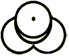
\includegraphics[scale=0.5]{images/motb}\footnotemark}\footnotetext{This image is thanks to Thelemapedia, a great resource for all things Thelema. Their images are released under the GNU Free Documentation license; this book has a compatible licensing scheme. -- \textsc{Editor.}}, and cry AIWAZ!

20. Let him trace the Invoking Hexagram of The Beast\footnote{Invoking Hexagram of the Beast: \unicursalhexagram{.5}}.

21. Let him lower the Wand, striking the Earth therewith.

22. Let him give the sign of Mater Triumphans. (The feet are together; the left arm is curved as if it supported a child; the thumb and index finger of the right hand pinch the nipple of the left breast, as if offering it to that child.) Let him utter the word \textgreek{ΘΕΛΕΜΑ}!

23. Perform the Spiral Dance, moving deosil and whirling widdershins. Each time on passing the West extend the Wand to the Quarter in question, and bow:

\begin{enumerate}[label=\alph*.]
\item \enquote{Before me the powers of LA!} (to West.)
\item \enquote{Behind me the powers of AL!} (to East.)
\item \enquote{On my right hand the powers of LA!} (to North.)
\item \enquote{On my left hand the powers of AL!} (to South.)
\item \enquote{Above me the powers of ShT!} (leaping in the air.)
\item \enquote{Beneath me the power of ShT!} (striking the ground.)
\item \enquote{Within me the Powers!} (in the attitude of Phthah erect, the feet together, the hands clasped upon the vertical Wand.)
\item \enquote{About me flames my Father's Face, the Star of Force and Fire!}
\item \enquote{And in the Column stands His six-rayed Splendour!}
\end{enumerate}

(This dance may be omitted, and the whole utterance chanted in the attitude of Phthah.)

\addsec*{The Final Gesture}

This is identical to the first gesture.

\raggedbottom\pagebreak

(Here followeth an impression of the ideas implied in this Paean.)


I also am a Star in Space, unique and self-existent, an individual
essence incorruptible; I also am one Soul; I am identical with All
and None. I am in All and all in Me; I am, apart from all and
lord of all, and one with all.

I am a God, I very God of very God; I go upon my way to work my will; I have made matter and motion for my mirror; I have decreed for my delight that Nothingness should figure itself as twain, that I might dream a dance of names and natures, and enjoy the substance of simplicity by watching the wanderings of my shadows. I am not that which is not; I know not that which knows not; I love not that which loves not. For I am Love, whereby division dies in delight; I am Knowledge, whereby all parts, plunged in the whole, perish and pass into perfection; and I am that I am, the being wherein Being is lost in Nothing, nor deigns to be but its Will to unfold its nature, its need to express its perfection in all possibilities, each phase a partial phantasm, and yet inevitable and absolute.

I am Omniscient, for naught exists for me unless I know it. I am Omnipotent, for naught occurs save by Necessity my soul's expression through my Will to be, to do, to suffer the symbols of itself. I am Omnipresent, for naught exists where I am not, who fashioned space as a condition of my consciousness of myself, who am the centre of all, and my circumference the frame of mine own fancy.

I am the All, for all that exists for me is a necessary expression in thought of some tendency of my nature, and all my thoughts are only the letters of my Name.

I am the One, for all that I am is not the absolute All, and all my all is mine and not another's; mine, who conceive of others like myself in essence and truth, yet unlike in expression and illusion.

I am the None, for all that I am is the imperfect image of the perfect; each partial phantom must perish in the clasp of its counterpart, each form fulfil itself by finding its equated opposite, and satisfying its need to be the Absolute by the attainment of annihilation.

The word, LAShTAL includes all this.

\textit{LA} \textemdash{} Naught.

\textit{AL} \textemdash{} Two.

\textit{L} is \enquote{Justice}, the Kteis fulfilled by the Phallus, \enquote{Naught and Two} because the plus and the minus have united in \enquote{love under will}.

\textit{A} is \enquote{The Fool}, Naught in Thought (Parzival), Word (Harpocrates), and Action (Bacchus). He is the boundless air, and the wandering Ghost, but with \enquote{possibilities}. He is the Naught that the Two have made by \enquote{love under will}.

\textit{LA} thus represents the Ecstasy of Nuit and Hadit conjoined, lost in love, and making themselves Naught thereby. Their child is begotten and conceived, but is in the phase of Naught also, as yet. LA is thus the Universe in that phase, with its potentialities of manifestation.

\textit{AL}, on the contrary, though it is essentially identical with LA, shows the Fool manifested through the Equilibrium of Contraries. The weight is still nothing, but it is expressed as it were two equal weights in opposite scales. The indicator still points to zero.

\textit{ShT} is equally 31 with \textit{LA} and \textit{AL}, but it expresses the secret nature which operates the Magick or the transmutations.

\textit{ShT} is the formula of this particular \AE{}on; another \ae{}on might have another way of saying 31.

\textit{Sh} is Fire as T is Force; conjoined they express Ra-Hoor-Khuit.

\enquote{The Angel} represents the St\'{e}l\'{e} 666, showing the Gods of the \AE{}on, while \enquote{Strength} is a picture of Babalon and the Beast, the earthly emissaries of those Gods.

\textit{ShT} is the dynamic equivalent of \textit{LA} and \textit{AL}. \textit{Sh} shows the Word of the Law, being triple, as 93 is thrice 31. \textit{T} shows the formula of Magick declared in that Word; the Lion, the Serpent, the Sun, Courage and Sexual Love are all indicated by the card.

In \textit{LA} note that Saturn or Satan is exalted in the House of Venus or Astarte and it is an airy sign. Thus \textit{L} is Father-Mother, Two and Naught, and the Spirit (Holy Ghost) of their Love is also Naught. Love is AHBH, 13, which is AChD. Unity, 1, Aleph. who is The Fool who is Naught, but none the less an individual One, who (as such) is not another, yet unconscious of himself until his Oneness expresses itself as a duality.

Any impression or idea is unknowable in itself. It can mean nothing until brought into relation with other things. The first step is to distinguish one thought from another; this is the condition of recognising it. To define it, we must perceive its orientation to all our other ideas. The extent of our knowledge of any one thing varies therefore with the number of ideas with which we can compare it. Every new fact not only adds itself to our universe, but increases the value of what we already possess.

In \textit{AL} this \enquote{The} or \enquote{God} arranges for \enquote{Countenance to behold countenance}, by establishing itself as an equilibrium, \textit{A} the One-Naught conceived as \textit{L} the Two-Naught. This \textit{L} is the Son-Daughter Horus-Harpocrates just as the other \textit{L} was the Father-Mother Set-Isis. Here then is Tetragrammaton once more, but expressed in identical equations in which every term is perfect in itself as a mode of Naught.

\textit{ShT} supplies the last element; making the Word of either five or six letters, according as we regard ShT as one letter or two. Thus the Word affirms the Great Work accomplished: $5^{\circ}=6^{\square}$.

\textit{ShT} is moreover a necessary resolution of the apparent opposition of \textit{LA} and \textit{AL}; for one could hardly pass to the other without the catalytic action of a third identical expression whose function should be to transmute them. Such a term must be in itself a mode of Naught, and its nature cannot encroach on the perfections of Not-Being, \textit{LA}, or of Being, \textit{AL}. It must be purely Nothing-Matter, so as to create a Matter-in-Motion which is a function of \enquote{Something}.

Thus \textit{ShT} is Motion in its double phase, an inertia compose of two opposite current, and each current is also thus polarised. \textit{Sh} is Heaven and Earth, \textit{T} Male and Female; \textit{ShT} is Spirit and Matter; one is the word of Liberty and Love flashing its Light to restore Life to Earth, the other is the act by which Life claims that Love is Light and Liberty. And these are Two-in-One, the divine letter of Silence-in-Speech whose symbol is the Sun in the arms of the Moon.

But \textit{Sh} and \textit{T} are alike formul\ae{} of force in action as opposed to entities; they are not states of existence, but modes of motion. They are verbs, not nouns.

\textit{Sh} is the Holy Spirit as a \enquote{tongue of fire} manifest in triplicity, and is the child of Set-Isis as their logos or Word uttered by their \enquote{Angel.} The card is XX, and 20 is the value of Yod (the Angel or Herald) expressed in full as IVD. \textit{Sh} is the spiritual congress of Heaven and Earth.

But \textit{T} is the Holy Spirit in action as a \enquote{roaring lion} or as the \enquote{old Serpent} instead of an \enquote{Angel of Light}. The twins of Set-Isis, harlot and beast, are busy with that sodomitic and incestuous lust which is the traditional formula for producing demi-gods, as in the cases of Mary and the Dove, Leda and the Swan, etc. The card is XI, the number of Magick AVD: Aleph the Fool impregnating the woman according to the Word of Yod, the Angel of the Lord! His sister has seduced her brother Beast, shaming the Sun with her sin; she has mastered the Lion, and enchanted the Serpent. Nature is outraged by Magick; man is bestialised and woman defiled. The conjunction produces a monster; it affirms regression of types. Instead of a man-God conceived of the Spirit of God by a virgin in innocence, we are asked to adore the bastard of a whore and a brute, begotten in shamefullest sin and born in most blasphemous bliss.

This is in fact the formula of our Magick; we insist that all acts must be equal; that existence asserts the right to exist; that unless evil is a mere term expressing some relation of haphazard hostility between forces equally self-justified, the universe is as inexplicable and impossible as uncompensated action; that the orgies of Bacchus and Pan are no less sacramental than the Masses of Jesus; that the scars of syphilis are sacred and worthy of honour as much as the wounds of the martyrs of Mary.

It should be unnecessary to insist that the above ideas apply only to the Absolute. Toothache is still painful, and deceit degrading, to a man, relatively to his situation in the world of illusion; he does his Will by avoiding them. But the existence of \enquote{Evil} is fatal to philosophy so long as it is supposed to be independent of conditions; and to accustom the mind to \enquote{make no difference} between any two ideas as such is to emancipate it from the thralldom of terror.

We affirm on our altars our faith in ourself and our wills, our love of all aspects of the Absolute All.

And we make the Spirit Shin combine with the Flesh Teth in a single letter, whose value is 31 even as those of \textit{LA} the Naught, and \textit{AL} the All, to complete their Not-Being and Being with its Becoming, to mediate between identical extremes as their mean \textemdash{} the secret that sunders and seals them.

It declares that all somethings are equally shadows of Nothing, and justifies Nothing in its futile folly of pretending that something is stable, by making us aware of a method of Magick through the practice of which we may partake in the pleasure of the process.

The Magician should devise for himself a definite technique for destroying \enquote{evil}. The essence of such a practice will consist in training the mind and the body to confront things which case fear, pain, disgust\footnote{The People of England have made two revolutions to free themselves from Popish fraud and tyranny. They are at their tricks again; and if we have to make a Third Revolution, let us destroy the germ itself!}, shame and the like. He must learn to endure them, then to become indifferent to them, then to become indifferent to them, then to analyse them until they give pleasure and instruction, and finally to appreciate them for their own sake, as aspects of Truth. When this has been done, he should abandon them, if they are really harmful in relation to health and comfort. Also, our selection of \enquote{evils} is limited to those that cannot damage us irreparable. E.g., one ought to practice smelling assaf\oe{}tida until one likes it; but not arsine or hydrocyanic acid. Again, one might have a liaison with an ugly old woman until one beheld and loved the star which she is; it would be too dangerous to overcome the distaste for dishonesty by forcing oneself to pick pockets. Acts which are essentially dishonourable must not be done; they should be justified only by calm contemplation of their correctness in abstract cases.

Love is a virtue; it grows stronger and purer and less selfish by applying it to what it loathes; but theft is a vice involving the slave-idea that one's neighbour is superior to oneself. It is admirable only for its power to develop certain moral and mental qualities in primitive types, to prevent the atrophy of such faculties as our own vigilance, and for the interest which it adds to the \enquote{tragedy, Man}.

Crime, folly, sickness and all such phenomena must be contemplated with complete freedom from fear, aversion, or shame. Otherwise we shall fail to see accurately, and interpret intelligently; in which case we shall be unable to outwit and outfight them. Anatomists and physiologists, grappling in the dark with death, have won hygiene, surgery, prophylaxis and the rest for mankind. Anthropologists, arch\ae{}ologists, physicists and other men of science, risking thumbscrews, stake, infamy and ostracism, have torn the spider-snare of superstition to shreds and broken in pieces the monstrous idol of Morality, the murderous Moloch which has made mankind its meat throughout history. Each fragment of that coprolite it manifest as an image of some brute lust, some torpid dullness, some ignorant instinct, or some furtive fear shapen in his own savage mind.

Man is indeed not wholly freed, even now. He is still trampled under the hoofs of the stampeding mules that nightmare bore to his wild ass, his creative forces that he had not mastered, the sterile ghosts that he called gods. Their mystery cows men still; they fear, they flinch, they dare not face the phantoms. Still, too, the fallen fetich seems awful; it is frightful to them that there is no longer an idol to adore with anthems, and to appease with the flesh of their firstborn. Each scrambles in the bloody mire of the floor to snatch some scrap for a relic, that he may bow down to it and serve it.

So, even to-day, a mass of maggots swarm heaving over the carrion earth, a brotherhood bound by blind greed for rottenness. Science still hesitates to raze the temple of Rimmon, though every year finds more of her sons impatient of Naaman's prudence. The Privy Council of the Kingdom of Mansoul sits in permanent secret session; it dares not declare what must follow its deed in shattering the monarch Morality into scraps of crumbling conglomerate of of climatic, tribal, and person prejudices, corrupted yet more by the action of crafty ambition, insane impulse, ignorant arrogance, superstitious hysteria, fear fashioning falsehoods on the stone that it sets on the grave of Truth whom it has murdered and buried in the black earth Oblivion. Moral philosophy, psychology, sociology, anthropology, mental pathology, physiology, and many another of the children of Wisdom, of whom she is justified, well know that the laws of Ethics are a chaos of confused conventions, based at best on customs convenient in certain conditions, more often on the craft or caprice of the biggest, the most savage, heartless, cunning and blood-thirsty brutes of the pack, to secure their power or pander to their pleasure in cruelty. There is no principle, even a false one, to give coherence to the clamour of ethical propositions. Yet the very men that have smashed Moloch, and strewn the earth with shapeless rubble, grow pale when they so much as whisper among themselves: \enquote{While Moloch ruled all men were bound by one law, and by the oracles of them that, knowing the fraud, feared not, but were his priests and wardens of his mystery. What now? How can any of us, though wise and strong as never was known, prevail on men to act in concert, now that each prays to his own chip of God, and yet knows every other chip to be a worthless ort, dream-dust, ape-dung, tradition-bone, or \textemdash{} what not else?}

So Science begins to see that the Initiates were maybe not merely silly and selfish in making their rule of silence, and in protecting Philosophy from the profane. Yet still she hopes that the mischief may not prove mortal, and begs that things may go on much as usual until that secret session decide on some plan of action.

It has always been fatal when somebody finds out too much too suddenly. If John Huss had cackled more like a hen, he might have survived Michaelmas, and been esteemed for his eggs. The last fifty years have laid the axe of analysis to the root of every axiom; they are triflers who content themselves with lopping the blossoming twigs of our beliefs, or the boughs of our intellectual instruments. We can no longer assert any single proposition, unless we guard ourselves by enumerating countless conditions which must be assumed.

This digression has outstayed its welcome; it was only invited by Wisdom that it might warn Rashness of the dangers that encompass even Sincerity, Energy and Intelligence when they happen not to contribute to Fitness\-/in\-/their\-/environment.

The Magician must be wary in his use of his powers; he must may every act not only accord with his Will, but with the properties of his position at the time. It might be my Will to reach the foot of a cliff; but the easiest way \textemdash{} also the speediest, most direct least obstructed, the way of minimum effort \textemdash{} would be simply to jump. I should have destroyed my Will in the act of fulfilling it, or what I mistook for it; for the True Will has no goal; its nature being to Go. Similarly, a parabola is bound by one law which fixes its relations with two straight lines at every point; yet it has no end short of infinity, and it continually changes its direction. The Initiate who is aware Who he is can always check is conduct by reference to the determinants of his curve, and calculate his past, his future, his bearings, and his proper course at any assigned moment; he can even comprehend himself as a simple idea. He may attain to measure fellow-parabolas, ellipses that cross his path, hyperbolas that span all space with their twin wings. Perhaps he may come at long last, leaping beyond the limits of his own law, to conceive that sublimely stupendous outrage to Reason, the Cone! Utterly inscrutable to him, he is yet well aware that he exists in the nature thereof, that he is necessary thereto, that he is ordered thereby, and that therefrom he is sprung, from the loins of so fearful a Father! His own infinity becomes zero in relation to that of the least fragment of the solid. He hardly exists at all. Trillions multiplied by trillions of trillions of such as he could not cross the frontier even of breadth, the idea which he came to guess at only because he felt himself bound by some mysterious power. Yet breadth is equally a nothing in the presence of the Cone. His first conception must evidently be a frantic spasm, formless, insane, not to be classed as an articulate thought. Yet, if he develops the faculties of his mind, the more he knows of it the more he sees that its nature is identical with his own whenever comparison is possible.

The True Will is thus both determined by its equations, and free because those equation are simply its own name, spelt out fully. His sense of being under bondage comes from his inability to read it; his sense that evil exists to thwart him arises when he begins to learn to read, reads wrong, and is obstinate that his error is an improvement.

We know one thing only. Absolute existence, absolute motion, absolute direction, absolute simultaneity, absolute truth, all such ideas: they have not, and never can have, any real meaning. If a man in delirium tremens fell into the Hudson River, he might remember the proverb and clutch at an imaginary straw. Words such as \enquote{truth} are like that straw. Confusion of thought is concealed, and its impotence denied, by the invention. This paragraph opened with \enquote{We know}: yet, questioned, \enquote{we} make haste to deny the possibility of possessing, or even of defining, knowledge. What could be more certain to a parabola-philosopher that he could be approached in two ways, and two only? It would be indeed little less that the whole body of his knowledge, implied in the theory of his definition of himself, and confirmed by every single experience. He could receive impressions only be meeting A, or being caught up by B. Yet he would be wrong in an infinite number of ways. There are therefore Aleph-Zero possibilities that at any moment a man may find himself totally transformed. And it may be that our present dazzled bewilderment is due to our recognition of the existence of a new dimension of thought, which seems so \enquote{inscrutably infinite} and \enquote{absurd} and \enquote{immoral}, etc. \textemdash{} because we have not studied it long enough to appreciate that its laws are identical with our own, though extended to new conceptions. The discovery of radioactivity created a momentary chaos in chemistry and physics; but it soon led to a fuller interpretation of the old ideas. It dispersed many difficulties, harmonised many discords, and \textemdash{} yea, more! It shewed the substance of Universe as a simplicity of Light and Life, manners to compose atoms, themselves capable of deeper self-realisation through fresh complexities and organisations, each with its own peculiar powers and pleasures, each pursuing its path through the world where all things are possible. It revealed the omnipresence of Hadit identical with Himself, yet fulfilling Himself by dividing his interplay with Nuit into episodes, each form of his energy isolated with each aspect of Her receptivity, delight developing delight continuous from complex to complex. It was the voice of Nature awakening at the dawn of the \AE{}on, as Aiwaz uttered the Word of the Law of Thelema.

So also shall he who invoketh often behold the Formless Fire, with trembling and bewilderment; but if he prolong his meditation, he shall resolve it into coherent and intelligible symbols, and he shall hear the articulate utterance of that Fire, interpret the thunder thereof as a still small voice in his heart. And the Fire shall reveal to his eyes his own image in its own true glory; and it shall speak in his ears the Mystery that is his own right Name.

This then in the virtue of the Magick of The Beast 666, and the canon of its proper usage; to destroy the tendency to discriminate between any two things in theory, and in practice to pierce the veils of every sanctuary, pressing forward to embrace every image; for there is none that is not very Isis. The Inmost is one with the Inmost; yet the form of the One is not the form of the other; intimacy exacts fitness. He therefore who liveth by air, let him not be bold to breathe water. But mastery cometh by measure: to him who with labour, courage, and caution giveth his life to understand all that doth encompass him, and to prevail against it, shall be increase. \enquote{The word of Sin is Restriction}; seek therefore Righteousness, enquiring into Iniquity, and fortify thyself to overcome it.
